\documentclass[
headings=optiontohead,              % allows double headers
12pt,                               % fontsize 
DIV=13,                             % koma script diveider amount. tells koma how much of the site can be written to
twoside=false,                      % if set to true, automatically formats as book style with different left and right pages
open=right,                         % starting page on twosided texts 
BCOR=10mm,                          % correction that accounts for the center of the pages being glued in
toc=bibliographynumbered            % bibliography gets a number and is listed in the table of contents
]{scrreport}

\usepackage[utf8]{inputenc}                     % correct encoding of output, technically not needed anymore
\usepackage[T1]{fontenc}                        % correct encoding of output, technically not needed anymore
\usepackage[english]{babel}                     % font that supports English
\usepackage{upgreek}                            % non-cursive Greek letters
\usepackage[stretch=10,shrink=10,protrusion=true,expansion=true,final]{microtype} % prettier block format
\usepackage{hyperref}                           % links for everything
\usepackage{color}                              % allows for setting in different colors
\usepackage[autooneside=false,automark]{scrlayer-scrpage} % page-style with "Kolumnentitel" (title of current chapter is displayed at the top)
\usepackage{lmodern}                            % alternative font (better use libertinus)
\usepackage[sb]{libertinus}                     % use the font libertinus (needs to be installed from the web)
\usepackage[slantedGreek]{libertinust1math}     % math mode improvement for libertinus
\usepackage{siunitx}                            % physical units setting
\usepackage{icomma}                             % commas in lists get extra space if needed                        
\usepackage{amsfonts,amssymb,amstext,amsmath,amsthm} % better math mode (\mathrm and \text) and symbols
\usepackage{xspace}                             % works to improve own commands and provides "\xspace"-command, that puts a space if needed
\usepackage{ifthen}                             % more control over non-obligatory parameters
\usepackage{titling}                            % get title values as macros
\usepackage[onehalfspacing]{setspace}           % control the spacing between lines and in enumeration lists
\usepackage[backend=biber, style=phys, biblabel=brackets]{biblatex} % citations with "modern" backend and an physics-accepted citation style
\usepackage{graphicx}                           % work with graphics 
\usepackage{ragged2e}                           % ragged-commands (when no block format is wanted)
\usepackage{pdfpages}                           % allows including of pdfs into this pdf
\usepackage{booktabs}                           % better table formatting
\usepackage{multicol}                           % allows for the definition of multi-columns in tables
\usepackage{multirow}                           % allows for the definition of multirow-tables instead of just multicolumn
\usepackage{float}                              % provides the "H" option for forcing placement of a figure
\usepackage[section]{placeins}                  % provides the command "\FloatBarrier" to control the end of floatable regions for figures/tables
\usepackage{floatpag}                           % make it possible for float-pages to not have a page number
\usepackage{url}                                % sometimes needed by biblatex, technically no longer needed
\usepackage{minted}                             % nice code highlighting (needs Python Package to compile!!)
\usepackage{accents}                            % better control over accents
\usepackage{mathtools}                          % more math control possibilities
\usepackage[autostyle=true]{csquotes}           % context-sensitive-quotes -> quotation marks that are set correctly for the context

\usepackage{blindtext} % TODO remove

\title{Investigation of transformer architectures for geometrical graph structures and their application to two-dimensional spin systems} % TODO lookup title
\author{Jonas Kell}
\date{7$^\text{th}$ October 2022}

\graphicspath{{./images/}}              % custom paths for folders in that graphics can be found

\sisetup                                % setup for siunitx
{
detect-all,
locale=US,                              % language setup for siunitx
range-phrase={ \text{to} },             % word that is put into an si range
range-units = single,                 % better display of error ranges
per-mode=symbol-or-fraction,            % more dynamic frac usage in inline/displaymath mode
separate-uncertainty,                   % for better +- , \pm when including an error range 
}

\hypersetup
{
colorlinks=true,
linkcolor=dblue,                                    % dark blue linkcolor
urlcolor=dblue,                                     % dark blue linkcolor
citecolor=dblue,                                    % dark blue linkcolor
pdfauthor = {REDACTED},                           % write details into the expanded file properties
pdftitle = {Investigation of transformer architectures for geometrical graph structures},                         
pdfkeywords = {neural networks, graphs, ai, physics, quantum mechanics, transformers, machine learning},           
pdfsubject = {Bachelor Thesis}                      
}

\AtBeginDocument{
	\let\mathbb\relax
	\DeclareMathAlphabet\PazoBB{U}{fplmbb}{m}{n}
	\newcommand{\mathbb}{\PazoBB}
}       %more options to the \mathbb command

\setminted[]{
    xleftmargin=0cm,
    xrightmargin=0cm,
    frame=single,
    framesep=.25cm,
    linenos,
    tabsize=2,
    breaklines,
    breakafter=.],
    breakaftersymbolpre= ,
}           %configure the minted code-highlighting style

\addbibresource{literature.bib}              %initialize bibtex with correct file

\NiceMatrixOptions{
code-for-first-row = \color{dblue} ,
code-for-last-row = \color{dblue} ,
code-for-first-col = \color{dblue} ,
code-for-last-col = \color{dblue}
}
                                  % another file that holds the package/document configuration
\linespread{1.1}                                    % line-spacing can be controlled here

\clubpenalty10000                                   % Schusterjunge, orphan
\widowpenalty10000                                  % Hurenkind, Witwe
\displaywidowpenalty=10000                          % Make document obey stricter rules considering "Schusterjungen" and "Hurenkinder"
\renewcommand{\topfraction}{0.8}                    % allows for more chilled "text to image ratio" 
\renewcommand{\bottomfraction}{0.8}
\renewcommand{\textfraction}{0.1}
\renewcommand{\floatpagefraction}{0.8}

% \renewcaptionname{ngerman}{\figurename}{Abb.}       %"Figure" becomes "Fig." in English
\setcapindent{0cm}                                  %useful if image captions have multiple lines. Removers indentation below "Fig."
\setlength{\parindent}{0cm}                         %removes indentation at start of new paragraphs


%bibliography slots are redefined/modified here
\DeclareFieldFormat{journaltitle}{\textsl{#1}\isdot}
\DeclareFieldFormat{titlecase}{{#1}}


%COLORS
\definecolor{dblue}{rgb}{0,0,0.5}
\definecolor{dred}{rgb}{0.5,0,0}
\definecolor{dgrey}{rgb}{0.5,0.5,0.5}

%overwrite the coma-script definitions
\addtokomafont{pagehead}{\normalfont\color{dgrey}}                  %overwrite the coma-script definitions
\addtokomafont{sectioning}{\rmfamily\color{dblue}\boldmath}         %rmfamily puts headings in "normal" "serif-font" instead of "sans-serif"  boldmath ensures a bold math font in subscripts
\addtokomafont{captionlabel}{\bfseries\footnotesize}                %better Fig. format
\addtokomafont{caption}{\footnotesize}                          

%! hyphenation commonly used words can be spelled here to provide latex with the correct places to make line breaks
\hyphenation{Li-pid-mono-lage}

% headline spacing
\RedeclareSectionCommand[beforeskip=0cm,afterskip=1cm]{chapter}                                  % another file that holds format information
%! Ref-Commands 
\newcommand*{\fullref}[1]{\hyperref[{#1}]{\textit{\autoref*{#1} \nameref*{#1}}}}
\newcommand*{\fullpage}[1]{\hyperref[{#1}]{Seite \pageref*{#1}}}
\newcommand*{\fullpages}[1]{\hyperref[{#1}]{Seiten \pageref*{#1}ff}}

%! Math operators and other small conveniences
\newcommand\thickbar[1]{\accentset{\rule{.6em}{.8pt}}{#1}}
\DeclareMathOperator{\ggt}{ggT}
\DeclareMathOperator{\kgv}{kgV}
\DeclarePairedDelimiter\ceil{\lceil}{\rceil}
\DeclarePairedDelimiter\floor{\lfloor}{\rfloor}
\renewcommand*{\arraystretch}{0.8}

%! qm commands
\newcommand{\hamiltonian}{\ensuremath{\mathcal{H}}\xspace}
\newcommand{\up}{\ensuremath{\uparrow}\xspace}
\newcommand{\down}{\ensuremath{\downarrow}\xspace}
                                % another file that holds predefined commands


\begin{document}

% ! Bibliography, page numbering and Title setups
\thispagestyle{empty}                           % make sure title page is not numbered or anything else


\newcommand{\mail}{REDACTED}



\begin{titlepage}
\makebox[\textwidth][c]{
\includegraphics[width=0.5\textwidth]{logo_uni_augsburg.jpg}}
    
\color{dblue}

\begin{center}
    \vspace*{2cm}
    \Huge
    \textbf{\thetitle}

    \vspace*{1.5cm}
    \color{black}
    \textbf{Bachelor Thesis}

    \vspace*{1cm}
    \normalsize
    submitted by\\
    \LARGE
    \theauthor\\\vspace*{0.3cm}
    \normalsize
    on \thedate

    \vspace{1.8cm}
    \color{black}
    \emph{Augsburg University}\\
    \emph{Faculty of Applied Computer Science}\\
    \emph{Institute of Computer Science}\\
    \emph{Chair for Machine Learning \& Computer Vision}

    \vfill

    \begin{tabular}{rl}
        1$^\text{st}$ Corrector: &REDACTED\\
        2$^\text{nd}$ Corrector: &REDACTED\\
    \end{tabular}
\end{center}

\end{titlepage}
                               % include title-page
\cleardoublepage                                % make sure, that if double-page is active, to reset the double page counter
\pagestyle{scrheadings}                         % puts current chapters title into the header in small gray font
\pagenumbering{roman}                           % number the pages of the table of contents in roman numerals
\renewcommand{\contentsname}{Table of Contents} % title of table of contents
\tableofcontents                                % table of contents
\noindent\\\\

\addsec*{List of Abbreviations}
\begin{tabular}[h]{p{3cm}|l}
	Abbreviation & Meaning\\
	\hline
	NQS & Neural Quantum State\\
	VMC & Variational Monte Carlo\\
	DMC & Diffusion Monte Carlo\\
	nn & nearest neighbor\\
	nnn & next nearest neighbor\\
	sgd & stochastic gradient descent\\
	GPU & graphics processing unit\\
	ReLU & rectifier linear unit\\
	RBM & restricted Boltzmann machine\\
	fcl & fully connected layer\\
\end{tabular}
\newpage                                   % list of abbreviations, figures, etc
\cleardoublepage                                % make sure, that if double-page is active, to reset the double page counter
\pagenumbering{arabic}                          % number the pages of the main document in Arabic numerals

% After this, the redefinition of the "Kolumnentitel" takes place
\clearpairofpagestyles
\ihead{\leftmark}
\ohead{\Ifstr{\leftmark}{\rightmark}{}{\rightmark}}
\cfoot*{\pagemark}
% End of the "Kolumnentitel" redefinition


% ! Main Document Body
\chapter{Introduction}
\label{sec:introduction}
The first set of experiments will be on the image classification task.
The goal will be to compare the architectural advantages and drawbacks between multiple different kinds of metaformers.

Training was be performed on a subset of 100 classes from the \emph{ImageNet} dataset \cite{imagenetDataset}.
The accompanying code to replicate these experiments can be found on GitHub \cite{selfComputerScience}.

The neural networks, as well as the training and evaluation code were written in python.
The \emph{PyTorch} \cite{pytorchGithub} machine learning framework was used as a measure to efficiently define neural networks and lever the computational capabilities of parallelization via GPUs.

The main metaformer model was originally based on the vision transformer found in an implementation of \emph{DINO} \cite{dinoGithub}, was however heavily modified. 
A comparison between the stock DINO model and the modified version will be also performed.
This however is not supposed to be a direct discrediting of any of the models, as their main purposes do not exactly align.
Therefore one or the other may excel in specific tasks.
Also a comparison against a pre-implemented \emph{poolformer} \cite{poolformerGithub} will be performed.

The \emph{einops} package \cite{einopsGithub} is heavily used. It provides tensor operations, configurable with the \emph{Einstein notation} and simplifies the notation and subsequently readability.
Lastly, the implementation of the \emph{positional encoding} is provided by \cite{positionalEncodingGithub}.

\FloatBarrier
\chapter{Theory}
\label{sec:theory}
    \section{From the Point of Physics}
        \label{sec:theory-physics}
        The first set of experiments will be on the image classification task.
The goal will be to compare the architectural advantages and drawbacks between multiple different kinds of metaformers.

Training was be performed on a subset of 100 classes from the \emph{ImageNet} dataset \cite{imagenetDataset}.
The accompanying code to replicate these experiments can be found on GitHub \cite{selfComputerScience}.

The neural networks, as well as the training and evaluation code were written in python.
The \emph{PyTorch} \cite{pytorchGithub} machine learning framework was used as a measure to efficiently define neural networks and lever the computational capabilities of parallelization via GPUs.

The main metaformer model was originally based on the vision transformer found in an implementation of \emph{DINO} \cite{dinoGithub}, was however heavily modified. 
A comparison between the stock DINO model and the modified version will be also performed.
This however is not supposed to be a direct discrediting of any of the models, as their main purposes do not exactly align.
Therefore one or the other may excel in specific tasks.
Also a comparison against a pre-implemented \emph{poolformer} \cite{poolformerGithub} will be performed.

The \emph{einops} package \cite{einopsGithub} is heavily used. It provides tensor operations, configurable with the \emph{Einstein notation} and simplifies the notation and subsequently readability.
Lastly, the implementation of the \emph{positional encoding} is provided by \cite{positionalEncodingGithub}.

        \FloatBarrier
        \subsection{The Ground State Search}
        \label{sec:theory-groundstatesearch}
        This section is supposed to introduce the fundamentals of (many body) quantum physics.


        \subsection{The Ising Model}
        \label{sec:theory-ising}
        In this thesis, a special case of quantum system will be discussed. 
The \emph{Ising model}.
The model describes multiple \emph{spins} that are locked in place. 
A spin is a very special kind of angular momentum that is inherent to quantum mechanical particles.
It helps to imagine the spin as a tiny magnet, that is locked in place, but can freely rotate to react to to external/neighboring  magnetic fields. This is a very harsh oversimplification, but enough for our purposes.

The state of the \emph{many body wavefunction} can solely be described by the direction that each of the spins is pointing into. In this simplified case, only \emph{spin-$\frac{1}{2}$} particles are used. That means each spin at each position can only either be pointing \emph{up} \up or \emph{down} \down (in relation to the z-axis).

That means, that a system with $n=3$ spins (in arbitrary, but fixed position) can be represented like \ref{eq:spin-ising}. $\vec{s}_m$ is the direction of the spin vector, that can (in this case) be simplified to the z-axis contribution $s^z_m$ of the vector. The values con only be $\frac{1}{2}$ (\up) or $-\frac{1}{2}$ (\down).
In this case the spins at the positions 1 and 2 point up, the one at 3 points down.

\begin{equation}
    \label{eq:spin-ising}
    \ket{\vec{s}_1, \vec{s}_2, \vec{s}_3} \rightarrow \ket{s^z_{1}, s^z_{2}, s^z_{3}} = \ket{\tfrac{1}{2}, \tfrac{1}{2}, -\tfrac{1}{2}} = \ket{\up, \up, \down}
\end{equation}

The hamiltonian for the system is defined as \ref{eq:hamiltonian-ising}. $J_{i, j}$ is the \emph{coupling constant} between the lattice sites $i$ and $j$. $h_i$ is a measure for the external magnetic field (in x-direction) at the lattice site $i$. Often the terms each get multiplied with $-1$ (sing flip of $J$ and $h$) as per convention. This was not done in this case in order for the equation to reflect the code. The $\hat{s}^a_i$ are \emph{operators}, that measure the $s^a_i$ number of the wavefunction (possibly altering its state in the process).

\begin{equation}
    \label{eq:hamiltonian-ising}
    \hamiltonian = \sum\limits_{i, j} J_{i, j} \cdot \hat{s}^z_i \hat{s}^z_j + \sum\limits_{i} h_i \cdot \hat{s}^x_i
\end{equation}

\ref{eq:hamiltonian-ising-nn} is a simplification, that assumes homogeneous interaction constants $J$ and $h$ for all sites, as well as only allowing nearest neighbors ($\langle i, j\rangle$) to interact.

\begin{equation}
    \label{eq:hamiltonian-ising-nn}
    \hamiltonian =  J \cdot \sum\limits_{\langle i, j \rangle} \hat{s}^z_i \hat{s}^z_j + h \cdot \sum\limits_{i} \hat{s}^x_i
\end{equation}

In this form, a $J < 0$ leads to so-called \emph{ferromagnetic} interaction. With a $J > 0$ the interaction is called \emph{anti-ferromagnetic}. When $h \neq 0$, the model is called \emph{transverse field Ising model} \cite{isingBook}.

The model was first solved for a 1D chain by Ernst Ising in 1924 \cite*[]{isingFerromagnetismn}. He solved the ferromagnetic case without a transverse field (however with an additional field parallel to the z-direction). His solution was analytically derived, but already not trivial to come up with.
With the introduction of a transverse field and a more complex lattice structure than a linear chain, there doesn't exist an analytic solution to even the most simplified hamiltonian \ref{eq:hamiltonian-ising-nn}.

In order to be able to use the hamiltonian, a few rules about the interaction of the used operators and the wavefunction will be introduced. They represent only a small subset of the mathematics and focus only on the bare minimum needed to understand the problem as someone that is unfamiliar with quantum mechanics. 

The spin operators can be written in terms of the \emph{Pauli spin matrices} \cite{schwablQM}. This is only mentioned, because it reflects the implementation in the code. Note that in the code, the $\frac{1}{2}$ factors in \ref{eq:pauli-rules} are omitted for simplification. $i$ stands for the complex unit.

\begin{equation}
    \label{eq:pauli-rules}
    \hat{s}^x = \frac{1}{2} \cdot \sigma^x = \frac{1}{2} \cdot \left(\begin{matrix}
        0& 1 \\
        1& 0
    \end{matrix}\right) \quad
    \hat{s}^y = \frac{1}{2} \cdot \sigma^y = \frac{1}{2} \cdot \left(\begin{matrix}
        0& -i \\
        i& 0
    \end{matrix}\right) \quad
    \hat{s}^z = \frac{1}{2} \cdot \sigma^z = \frac{1}{2} \cdot \left(\begin{matrix}
        1& 0 \\
        0& -1
    \end{matrix}\right)
\end{equation}

With the corresponding Pauli representation of the spin vectors \ref{eq:pauli-vectors}, the interaction of the operators can be directly computed with standard matrix multiplication. The important ones are calculated in \ref{eq:pauli-transformation}.

\begin{equation}
    \label{eq:pauli-vectors}
    \ket{\up} = \left(\begin{matrix}
        1\\0
    \end{matrix}\right)
    \qquad
    \ket{\down} = \left(\begin{matrix}
        0\\1
    \end{matrix}\right)
\end{equation}


\begin{equation}
    \label{eq:pauli-transformation}
    \sigma^z \ket{\up} = +1 \cdot \ket{\up} \quad
    \sigma^z \ket{\down} = -1 \cdot \ket{\down} \quad
    \sigma^x \ket{\up} = +1 \cdot \ket{\down} \quad
    \sigma^x \ket{\down} = +1 \cdot \ket{\up}
\end{equation}

The last important piece of information is, that operators denoted by indices only interact with the spin at the corresponding lattice site. Three examples are given in \ref{eq:pauli-many-body}. Multiple operators acting on one state can be computed by only evaluating the effect of the rightmost operator according to the mentioned rules and then repeating until finished. Complex numbers can always be commutatively swapped with operators and bra-kets.

\begin{equation}
    \label{eq:pauli-many-body}
    \sigma^z_2 \ket{\down, \up, \down} = +1 \cdot \ket{\down, \up, \down} \quad
    \sigma^z_1 \ket{\down, \up, \down} = -1 \cdot \ket{\down, \up, \down} \quad
    \sigma^z_3 \ket{\down, \down, \down} = +1 \cdot \ket{\down, \down, \up}
\end{equation}  
        \FloatBarrier
        \FloatBarrier
        \subsection{Numerical Solution}
        \label{sec:theory-numericalsolution}
        \subsection{Solutions with Neural Quantum States}
        \label{sec:theory-neuralquantumstates}
        \subsection{Imaginary Time Evolution}
        \label{sec:theory-imagenarytimeevolution}
        \subsection{Explored Lattice Patterns}
        \label{sec:theory-latticepatterns}
    \section{From the Point of Computer Science}
        \label{sec:theory-cs}
        The first set of experiments will be on the image classification task.
The goal will be to compare the architectural advantages and drawbacks between multiple different kinds of metaformers.

Training was be performed on a subset of 100 classes from the \emph{ImageNet} dataset \cite{imagenetDataset}.
The accompanying code to replicate these experiments can be found on GitHub \cite{selfComputerScience}.

The neural networks, as well as the training and evaluation code were written in python.
The \emph{PyTorch} \cite{pytorchGithub} machine learning framework was used as a measure to efficiently define neural networks and lever the computational capabilities of parallelization via GPUs.

The main metaformer model was originally based on the vision transformer found in an implementation of \emph{DINO} \cite{dinoGithub}, was however heavily modified. 
A comparison between the stock DINO model and the modified version will be also performed.
This however is not supposed to be a direct discrediting of any of the models, as their main purposes do not exactly align.
Therefore one or the other may excel in specific tasks.
Also a comparison against a pre-implemented \emph{poolformer} \cite{poolformerGithub} will be performed.

The \emph{einops} package \cite{einopsGithub} is heavily used. It provides tensor operations, configurable with the \emph{Einstein notation} and simplifies the notation and subsequently readability.
Lastly, the implementation of the \emph{positional encoding} is provided by \cite{positionalEncodingGithub}.

        \FloatBarrier
        \subsection{The Image Classification Task}
        \label{sec:theory-imageclassification}
        \subsection{Neural Network Training}
        \label{sec:theory-neuralnetworktraining}
        \subsection{Neural Network Pre-Training}
        \label{sec:theory-pretraining}
        \subsection{Employment of Graphs for Problem transfer}
        \label{sec:theory-graphs}

\chapter{Machine Learning Architectures}
\label{sec:architectures}

    \section{Used Architectures}
        \subsection{Perceptron Architectures}
        \label{sec:architectures-perceptron}
        \subsection{Pooling}
        \label{sec:architectures-pooling}
        \subsection{Convolutional Architectures}
        \label{sec:architectures-convolution}
        \subsection{Attention and the Transformer}
        \label{sec:architectures-attention}
        \subsection{The Metaformer}
        \label{sec:architectures-metaformer}
        \subsection{Graph Architectures}
        \label{sec:architectures-graphs}
    \section{Usage of Inductive Biases}
        \subsection{Conventional Architectures}
        \label{sec:architectures-biasesnormal}
        \subsection{Metaformer Architectures}
        \label{sec:architectures-biasesmetaformer}
        \subsection{Graph Architectures}
        \label{sec:architectures-biasesgraph}

\chapter{Experiments and their Results}
    \section{Metaformer in Image Classification}
        \subsection{Training Settings}
        \label{sec:experiments-trainingsettings}

        \subsection{Importance of Positional Encoding}
        \label{sec:experiments-positionalencoding}
        \subsection{Comparison of different Token Mixers}
        \label{sec:experiments-tokenmixers}

    \section{Metaformer in Ground State Search}
        \subsection{Comparison to established Architectures}
        \label{sec:experiments-comparisontoestablished}
        \subsection{Resiliency to the Choice of Lattice Encoding}
        \label{sec:experiments-resiliencylatticeencoding}
        \subsection{Optimizing the Ansatz}
        \label{sec:experiments-optimizingtheansatz}
        \subsection{Choice of Hyperparameters}
        \label{sec:experiments-hyperparameters}
        \subsection{Differences across the Phase Diagram}
        \label{sec:experiments-phasecriticalpoint}

\chapter{Conclusion}
\label{sec:conclusion}

% ! Addendum
\newpage
\nocite{*}
\printbibliography[title={Bibliography}]
\chapter{Appendix}
\label{sec:appendix}

%! needs to be first, because of format adapted to chapter title of appendix
\section{Lattice Visualization} \label{appendix:lattice-visualisation}

\begin{minipage}{\linewidth}
    \centering
    \makebox[\textwidth][c]{
        \makebox[1.25\textwidth][c]{
            \makebox[0.40\textwidth][l]{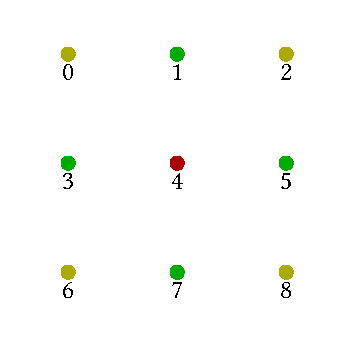
\includegraphics[width=0.33\textwidth]{./../appendix/lattice_visualization/square,size=2,np.pdf}}
            \makebox[0.40\textwidth][l]{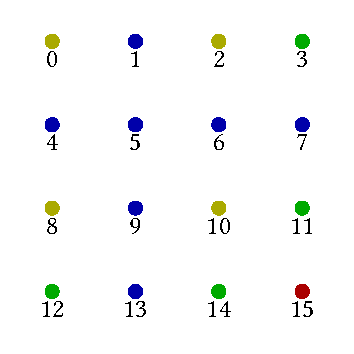
\includegraphics[width=0.33\textwidth]{./../appendix/lattice_visualization/square,size=3,p.pdf}}
            \makebox[0.40\textwidth][l]{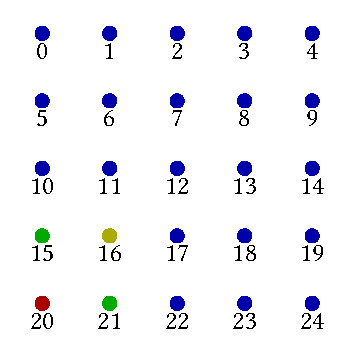
\includegraphics[width=0.33\textwidth]{./../appendix/lattice_visualization/square,size=4,np.pdf}}
        }
    }

    \captionof{figure}{A visualization of the \textbf{2D-square} lattice structure, measured in this thesis. 
        The lattices from left to right can be described by the parameters\\
        1: \emph{size=2, non-periodic}\,\,\,\, 2: \emph{size=3, periodic}\,\,\,\, 3: \emph{size=4, non-periodic}
    }
    \label{fig:appendix-square-lattices}
\end{minipage}

\vspace{0.5cm}

\begin{minipage}{\linewidth}
    \centering
    \makebox[\textwidth][c]{
        \makebox[1.25\textwidth][c]{
            \makebox[0.40\textwidth][l]{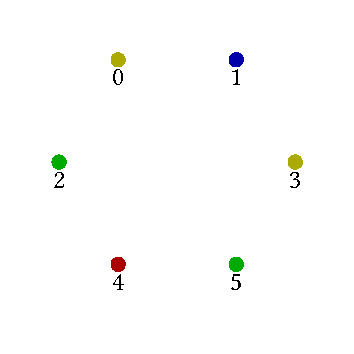
\includegraphics[width=0.33\textwidth]{./../appendix/lattice_visualization/hexagonal,size=1,np.pdf}}
            \makebox[0.40\textwidth][l]{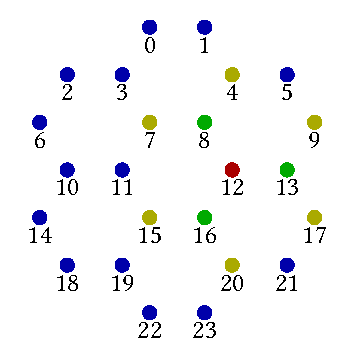
\includegraphics[width=0.33\textwidth]{./../appendix/lattice_visualization/hexagonal,size=2,np.pdf}}
            \makebox[0.40\textwidth][l]{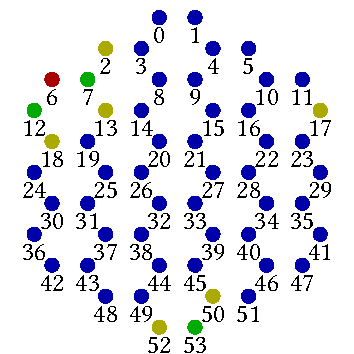
\includegraphics[width=0.33\textwidth]{./../appendix/lattice_visualization/hexagonal,size=3,p.pdf}}
        }
    }

    \vspace{0.3cm}
    \captionof{figure}{A visualization of the \textbf{2D-hexagonal} lattice structure, measured in this thesis. 
        The lattices from left to right can be described by the parameters \\
        1: \emph{size=1, non-periodic}\,\,\,\, 2: \emph{size=2, non-periodic}\,\,\,\, 3: \emph{size=3, periodic}
    }
    \label{fig:appendix-hexagonal-lattices}
\end{minipage}

\vspace{0.4cm}

\begin{minipage}{\linewidth}
    \centering
    \makebox[\textwidth][c]{
        \makebox[1.25\textwidth][c]{
            \makebox[0.40\textwidth][l]{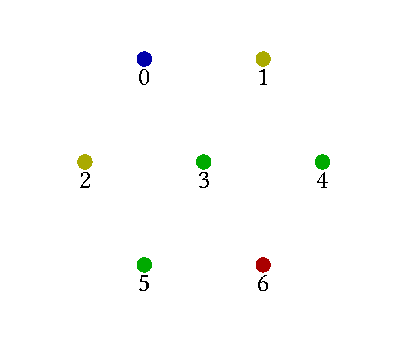
\includegraphics[width=0.33\textwidth]{./../appendix/lattice_visualization/trigonal_hexagonal,size=1,np.pdf}}
            \makebox[0.40\textwidth][l]{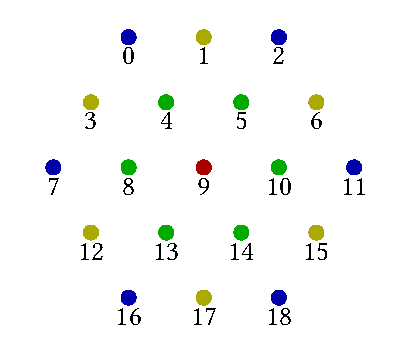
\includegraphics[width=0.33\textwidth]{./../appendix/lattice_visualization/trigonal_hexagonal,size=2,np.pdf}}
            \makebox[0.40\textwidth][l]{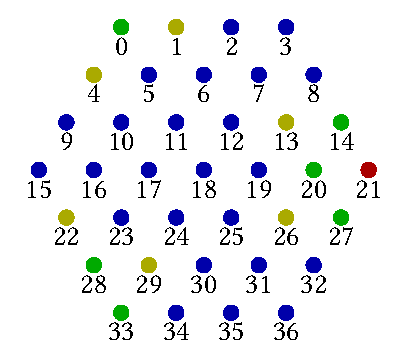
\includegraphics[width=0.33\textwidth]{./../appendix/lattice_visualization/trigonal_hexagonal,size=3,p.pdf}}
        }
    }
    
    \vspace{0.5cm}
    \captionof{figure}{A visualization of the \textbf{2D-trigonal\_hexagonal} lattice structure, measured in this thesis. 
        The lattices from left to right can be described by the parameters \\
        1: \emph{size=1, non-periodic}\,\,\,\, 2: \emph{size=2, non-periodic}\,\,\,\, 3: \emph{size=3, periodic}
    }
    \label{fig:appendix-trigonal_hexagonal-lattices}
\end{minipage}

% HERE SHOULD THE PAGE-BREAK BE. i love latex, but stuff like this infuriates me to get correct
\newpage
\makebox{\vspace{5cm}}\\

\begin{minipage}{\linewidth}
    \centering
    \makebox[\textwidth][c]{
        \makebox[1.25\textwidth][c]{
            \makebox[0.40\textwidth][l]{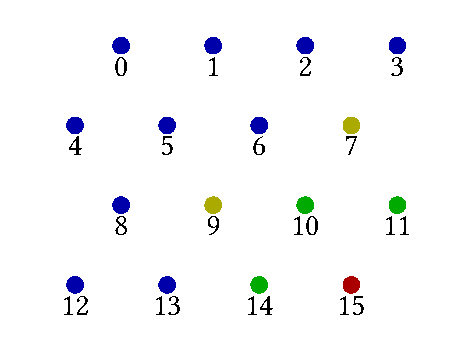
\includegraphics[width=0.33\textwidth]{./../appendix/lattice_visualization/trigonal_square,size=2,np.pdf}}
            \makebox[0.40\textwidth][l]{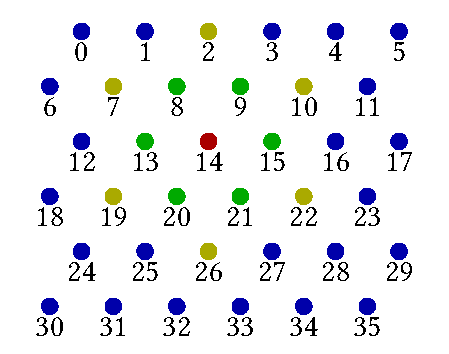
\includegraphics[width=0.33\textwidth]{./../appendix/lattice_visualization/trigonal_square,size=3,np.pdf}}
            \makebox[0.40\textwidth][l]{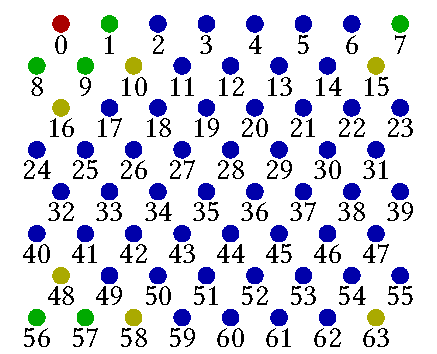
\includegraphics[width=0.33\textwidth]{./../appendix/lattice_visualization/trigonal_square,size=4,p.pdf}}
        }
    }

    \vspace{0.4cm}
    \captionof{figure}{A visualization of the \textbf{2D-trigonal\_square} lattice structure, measured in this thesis. 
        The lattices from left to right can be described by the parameters \\
        1: \emph{size=2, non-periodic}\,\,\,\, 2: \emph{size=3, non-periodic}\,\,\,\, 3: \emph{size=4, periodic}
    }
    \label{fig:appendix-trigonal_square-lattices}
\end{minipage}

\vspace{1.2cm}

\begin{minipage}{\linewidth}
    \centering
    \makebox[\textwidth][c]{
        \makebox[1.25\textwidth][c]{
            \makebox[0.40\textwidth][c]{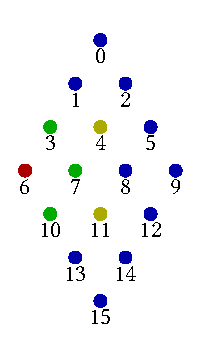
\includegraphics[width=0.20\textwidth]{./../appendix/lattice_visualization/trigonal_diamond,size=3,np.pdf}}
            \makebox[0.40\textwidth][c]{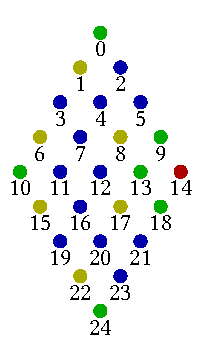
\includegraphics[width=0.20\textwidth]{./../appendix/lattice_visualization/trigonal_diamond,size=4,p.pdf}}
            \makebox[0.40\textwidth][c]{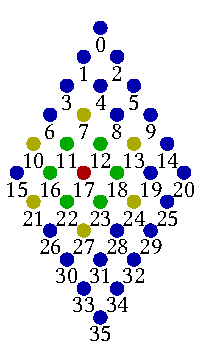
\includegraphics[width=0.20\textwidth]{./../appendix/lattice_visualization/trigonal_diamond,size=5,np.pdf}}
        }
    }

    \vspace{0.4cm}
    \captionof{figure}{A visualization of the \textbf{2D-trigonal\_diamond} lattice structure, measured in this thesis. 
        The lattices from left to right can be described by the parameters \\
        1: \emph{size=3, non-periodic}\,\,\,\, 2: \emph{size=4, periodic}\,\,\,\, 3: \emph{size=5, non-periodic}
    }
    \label{fig:appendix-trigonal_diamond-lattices}
\end{minipage}

\vspace{1.2cm}

\begin{minipage}{\linewidth}
    \centering
    \makebox[\textwidth][c]{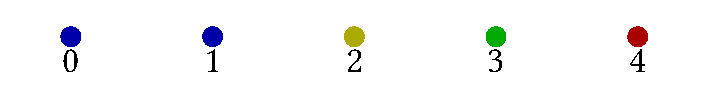
\includegraphics[width=0.80\textwidth]{./../appendix/lattice_visualization/linear,size=5,np.pdf}}
    \vspace*{0.2cm}
    \makebox[\textwidth][c]{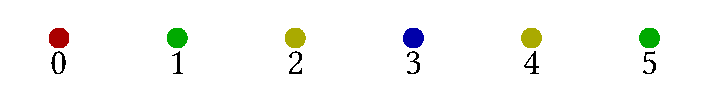
\includegraphics[width=0.80\textwidth]{./../appendix/lattice_visualization/linear,size=6,p.pdf}}
    \vspace*{0.2cm}
    \makebox[\textwidth][c]{
\includegraphics[width=0.80\textwidth]{./../appendix/lattice_visualization/linear,size=8,np.pdf}}

    \vspace{0.2cm}
    \captionof{figure}{A visualization of the \textbf{1D-linear} lattice structure, measured in this thesis. 
        The lattices from top to bottom can be described by the parameters \\
        1: \emph{size=5, non-periodic}\,\,\,\, 2: \emph{size=6, periodic}\,\,\,\, 3: \emph{size=8, non-periodic}
    }
    \label{fig:appendix-linear-lattices}
\end{minipage}

\newpage

% pdf as a additional information, can be nicely ref-ed ("\fullpage{anhang:test}") because of fake section that doesn't get shown in the table of contents
% \includepdf[pagecommand={\section*{} \label{appendix:test}}]{appendix/test.pdf}

% minted to properly import and style code. ! Needs python libraries
\newpage
\section{Dot Product Self Attention (jax)} \label{appendix:attention}
    \cite{selfPhysics}, \filepath{/models/metaformer.py}
    \inputminted[firstline=149, lastline=169]{python}{./../physics-code/models/metaformer.py}

\section{Graph Conformer Module (jax)} \label{appendix:graph-conformer}
    \cite{selfPhysics}, \filepath{/models/metaformer.py}
    \inputminted[firstline=242, lastline=284]{python}{./../physics-code/models/metaformer.py}

\newpage
\section{Graph Poolformer Module (jax)} \label{appendix:graph-poolformer}
    \cite{selfPhysics}, \filepath{/models/metaformer.py}
    \inputminted[firstline=211, lastline=239]{python}{./../physics-code/models/metaformer.py}
    

\end{document}





